\section{Efficiency calculations}
\label{sec:hhh:eff}

Although the normalization channels have the same final state particles, the efficiency does not
completely cancel due to kinematic differences.
Therefore the relative efficiency between signal and normalization decays must be calculated.
The efficiency for each decay is computed using simulated events, under the assumption that the
simulation accurately describes data, where there are discrepancies the simulations must be corrected.
%These efficiencies were calculated using simulated events; therefore, in order that the above
%efficiencies are correct it is imperative that the simulated events describe the data accurately.
%Where there are discrepancies, the simulations must be corrected.
There are some variables which are known to be poorly described in simulation, particularly track
multiplicity and the \chisqvtx of the \Bp candidate.
The effects of these discrepancies are minimized by reweighting simulated events using
the distributions of \btojpsikpipi.
Track multiplicity is known to be poorly described in simulation, generally there are fewer tracks
in simulation than observed in data,
these discrepancies are illustrated in \Fig{fig:hhh:ntracks}.
Aside from the direct differences, the low track multiplicity of in simulated events is a
contributing factor of \pid variables being badly described in simulations.

\begin{figure}[t]
  \begin{center}
    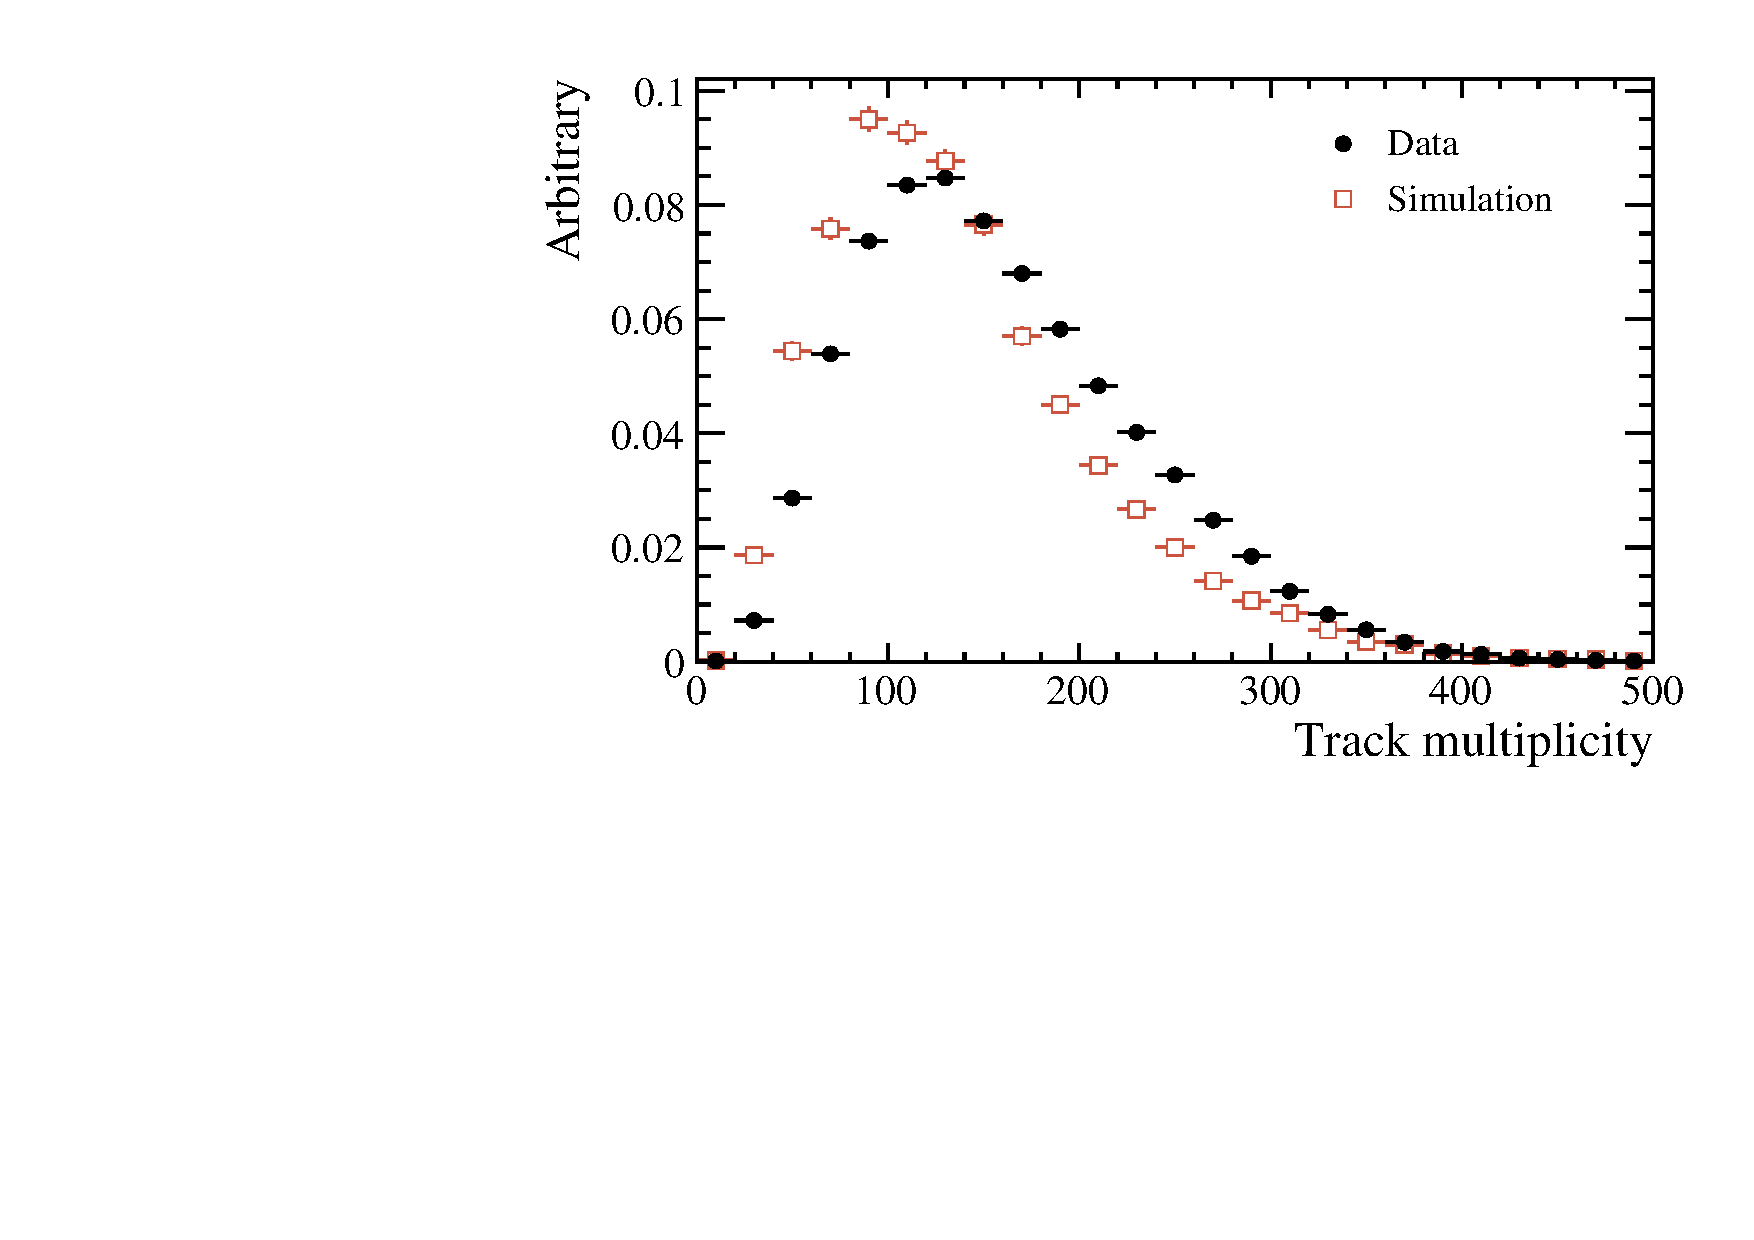
\includegraphics[width=0.48\textwidth]{ntracks}
    \caption[Comparison of track multiplicity between data and simulation]
    {
      Distributions of track multiplicity for (black circles) data and (red squares) simulation.
      Simulated events are known to mis-model the track multiplicity, having a lower average number
      of tracks per event.
    }
    \label{fig:hhh:ntracks}
  \end{center}
\end{figure}

To ensure that efficiencies from \pid cuts are determined accurately from simulation, the variables
must be corrected.
This is done using data driven methods, using highly pure samples of pions, kaons
and muons (coming from the decays \decay{\Dstarp}{\Dz(\to\kpi)\pip} and
\jpsitomumu).
For each hadron track in the simulated \Bp candidate, a new \pid variable is resampled from \pid
distributions of the pure track samples as a function of the track's pseudorapidity, momentum, and
track multiplicity.
Figure~\ref{fig:hhh:pid} shows the effect of this resampling technique, it is observed that the
simulated \pid distributions that have been resampled matches data distributions much better than the
raw distributions; the differences that remain are accounted for in the systematic uncertainties.
Muon \pid distributions are sufficiently well modelled in simulation that correcting them is
unnecessary.

\begin{figure}[t]
  \begin{center}
    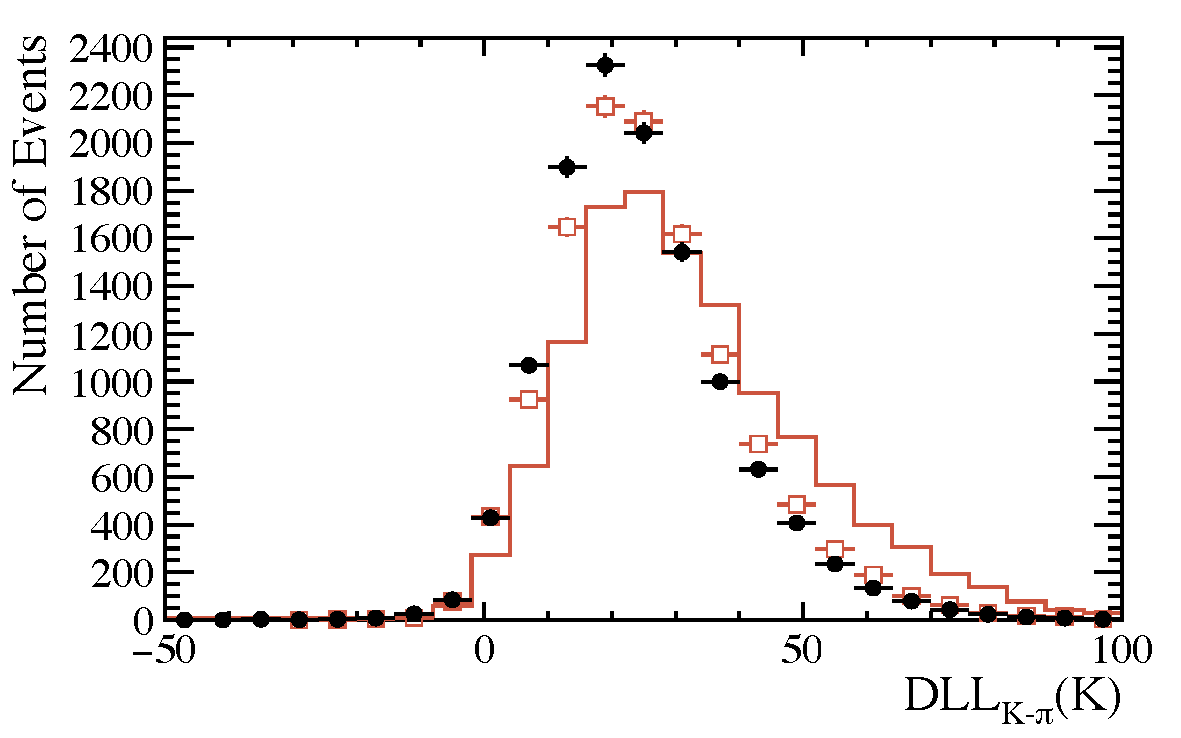
\includegraphics[width=0.48\textwidth]{pid_Kplus}
    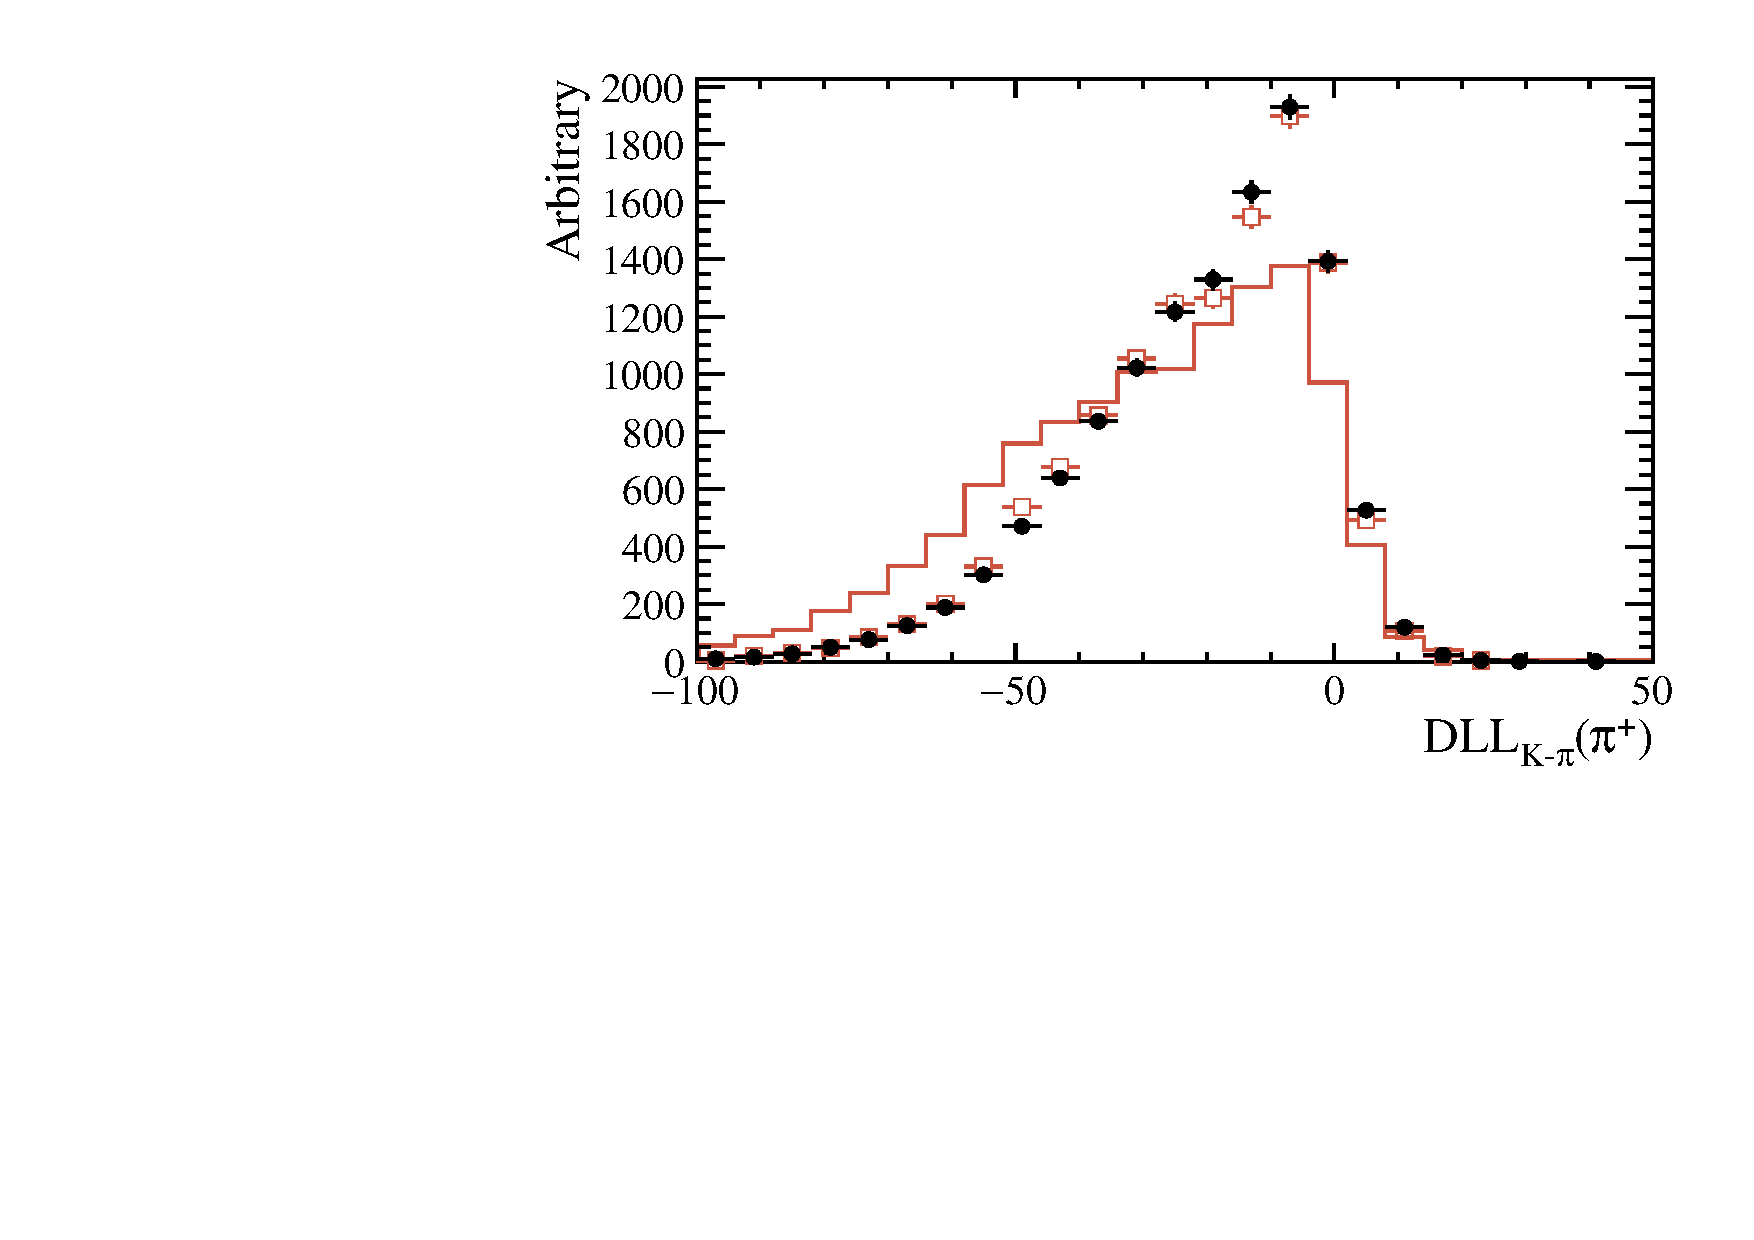
\includegraphics[width=0.48\textwidth]{pid_piplus}\\
    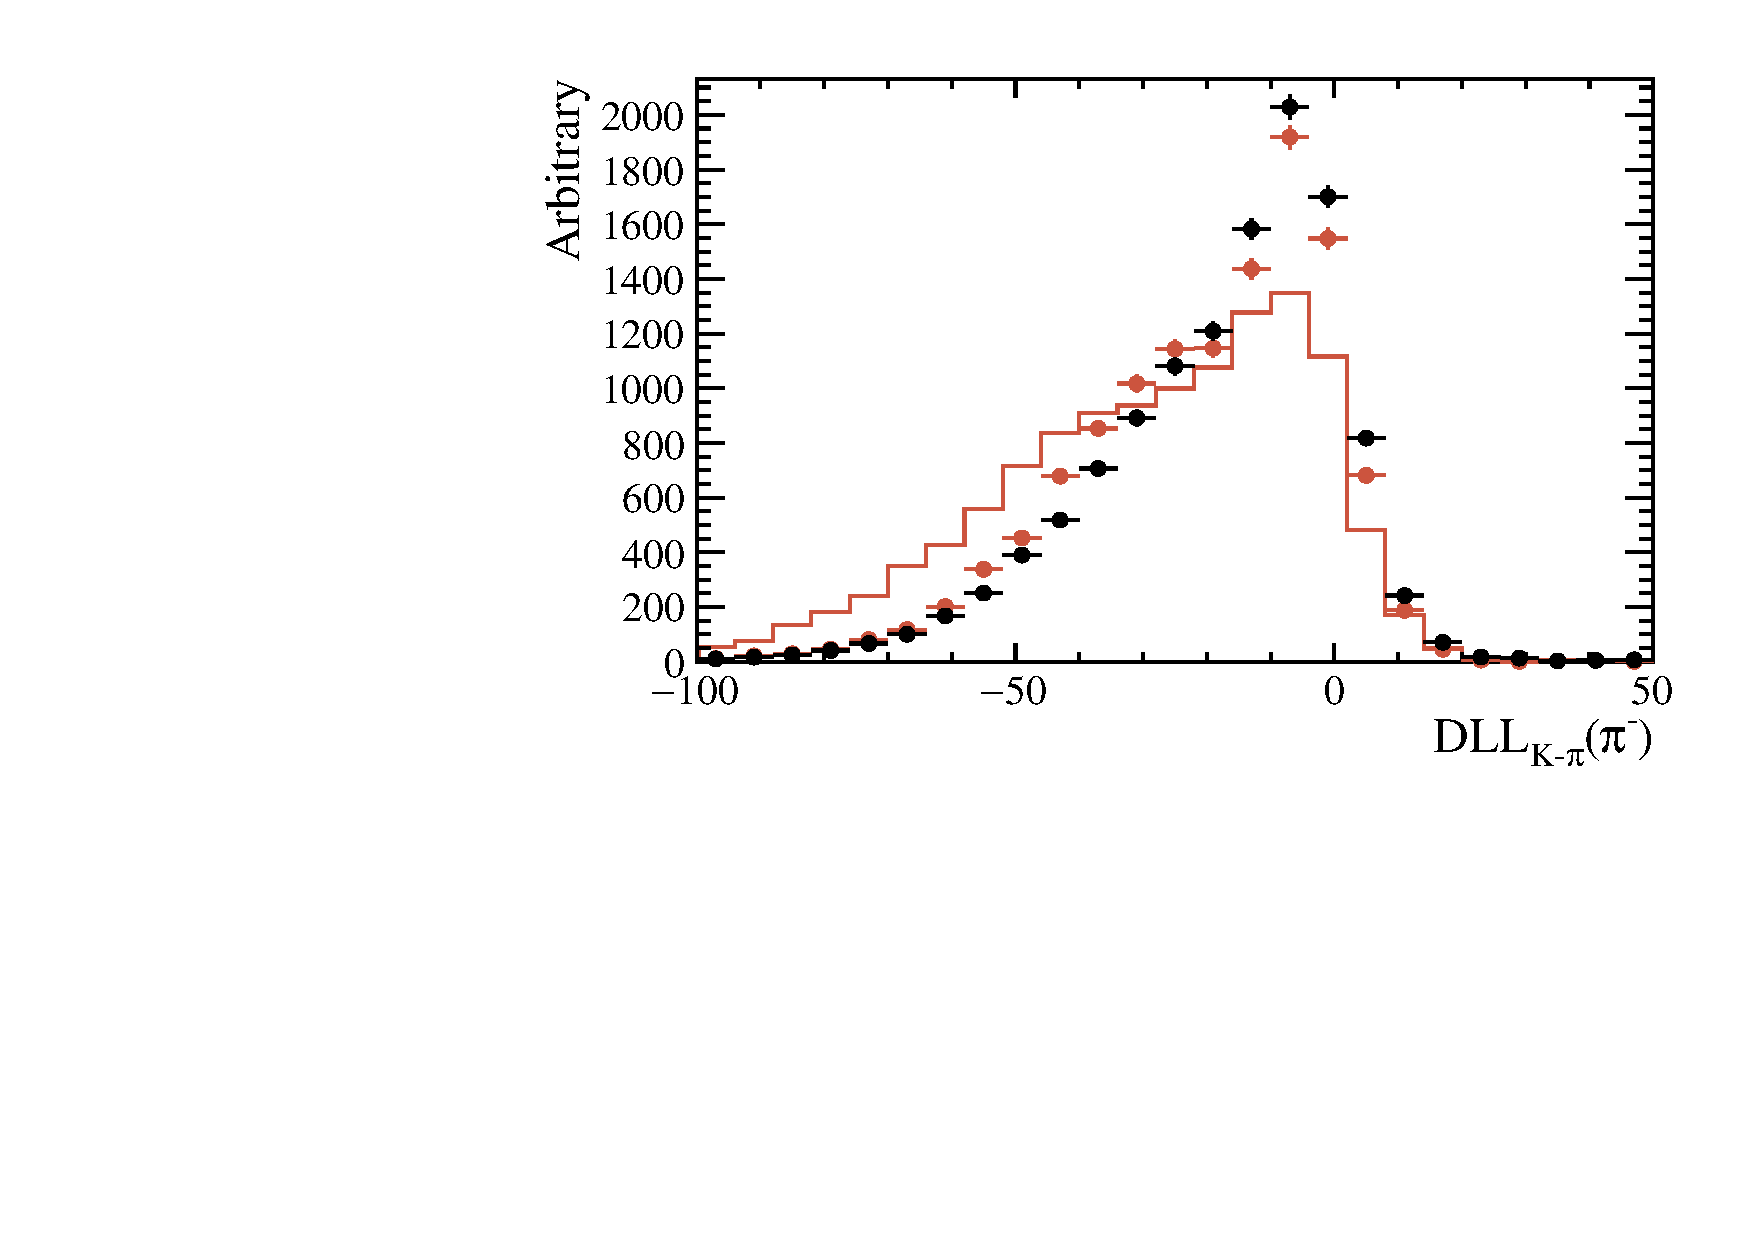
\includegraphics[width=0.48\textwidth]{pid_piminus}
    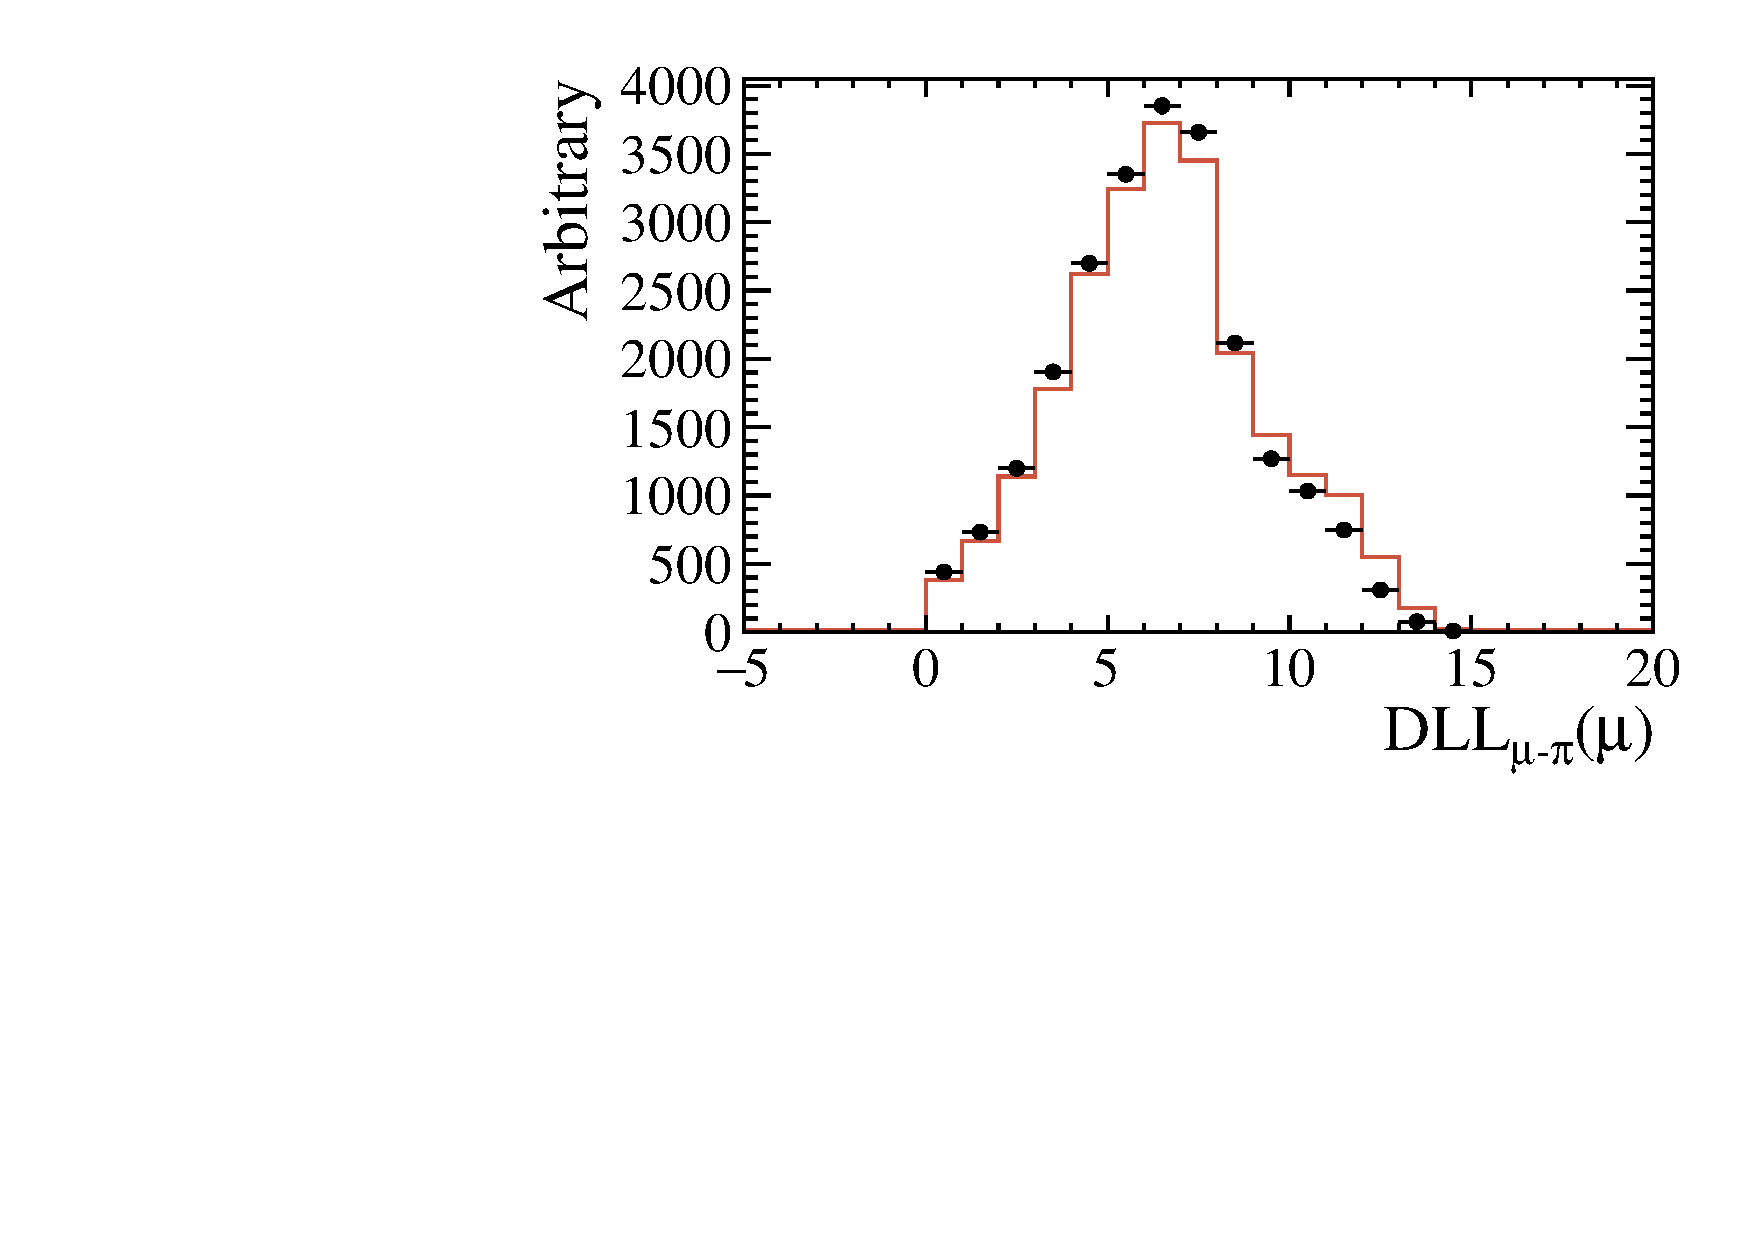
\includegraphics[width=0.48\textwidth]{pid_mu}
    \caption[Effect of resampling PID variables in simulation]
    {
      The effect of \pid resampling for simulated tracks using pure samples of particles for kaons
      and pions.
      There is marked improvement in the similarity of the (black circles) \btojpsikpipi data and
      simulated events before (red line) resampling and after (red squares).
      Muon candidates need not be resampled since muon \pid is well described in simulation.
      %\bam{MUON \pid PLOT}
    }
    \label{fig:hhh:pid}
  \end{center}
\end{figure}

%Reweighting

Tracking efficiency varies depending upon the regions of the detector through which the particle
passes, and the modelling of the detector in the simulation behaves differently to in actuality.
To correct for this, each candidate is weighted based on the relative tracking efficiency between
data and simulation, this is dependent upon $p$ and $\eta$.
The same is true for the response of the \ismuon variable.
Figure~\ref{fig:hhh:trackeff} shows how the tracking efficiency and \ismuon criteria are corrected
for throughout the detector volume.
After all reweighting all the aforementioned variables in simulated events, the \BDT distributions
are seen to be in agreement, this is shown in \Fig{fig:kpipi:bdt}.
%Geometric efficiencies
%Tracking efficiencies and isMuon
%Geometric efficiencies

\begin{figure}[t]
  \begin{center}
    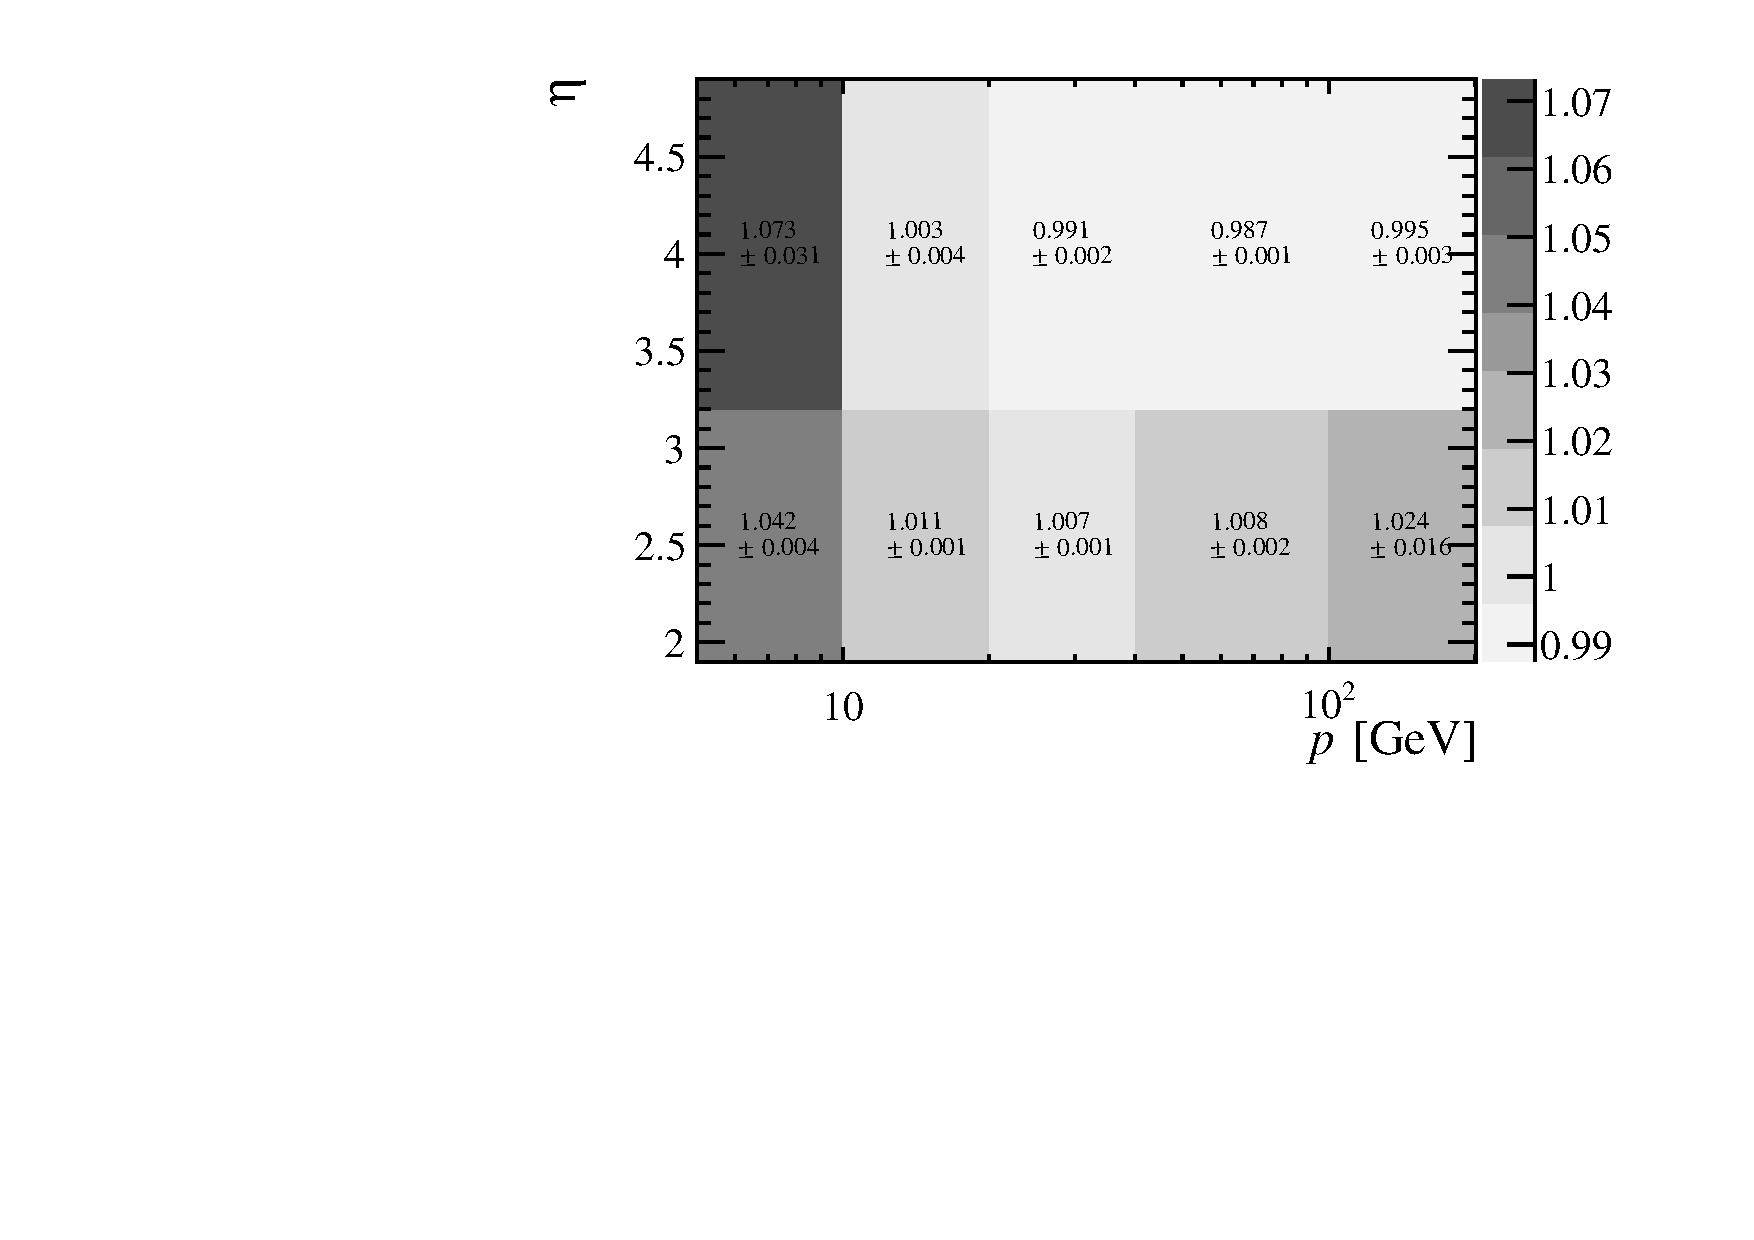
\includegraphics[height=0.23\textheight]{trackeff}
    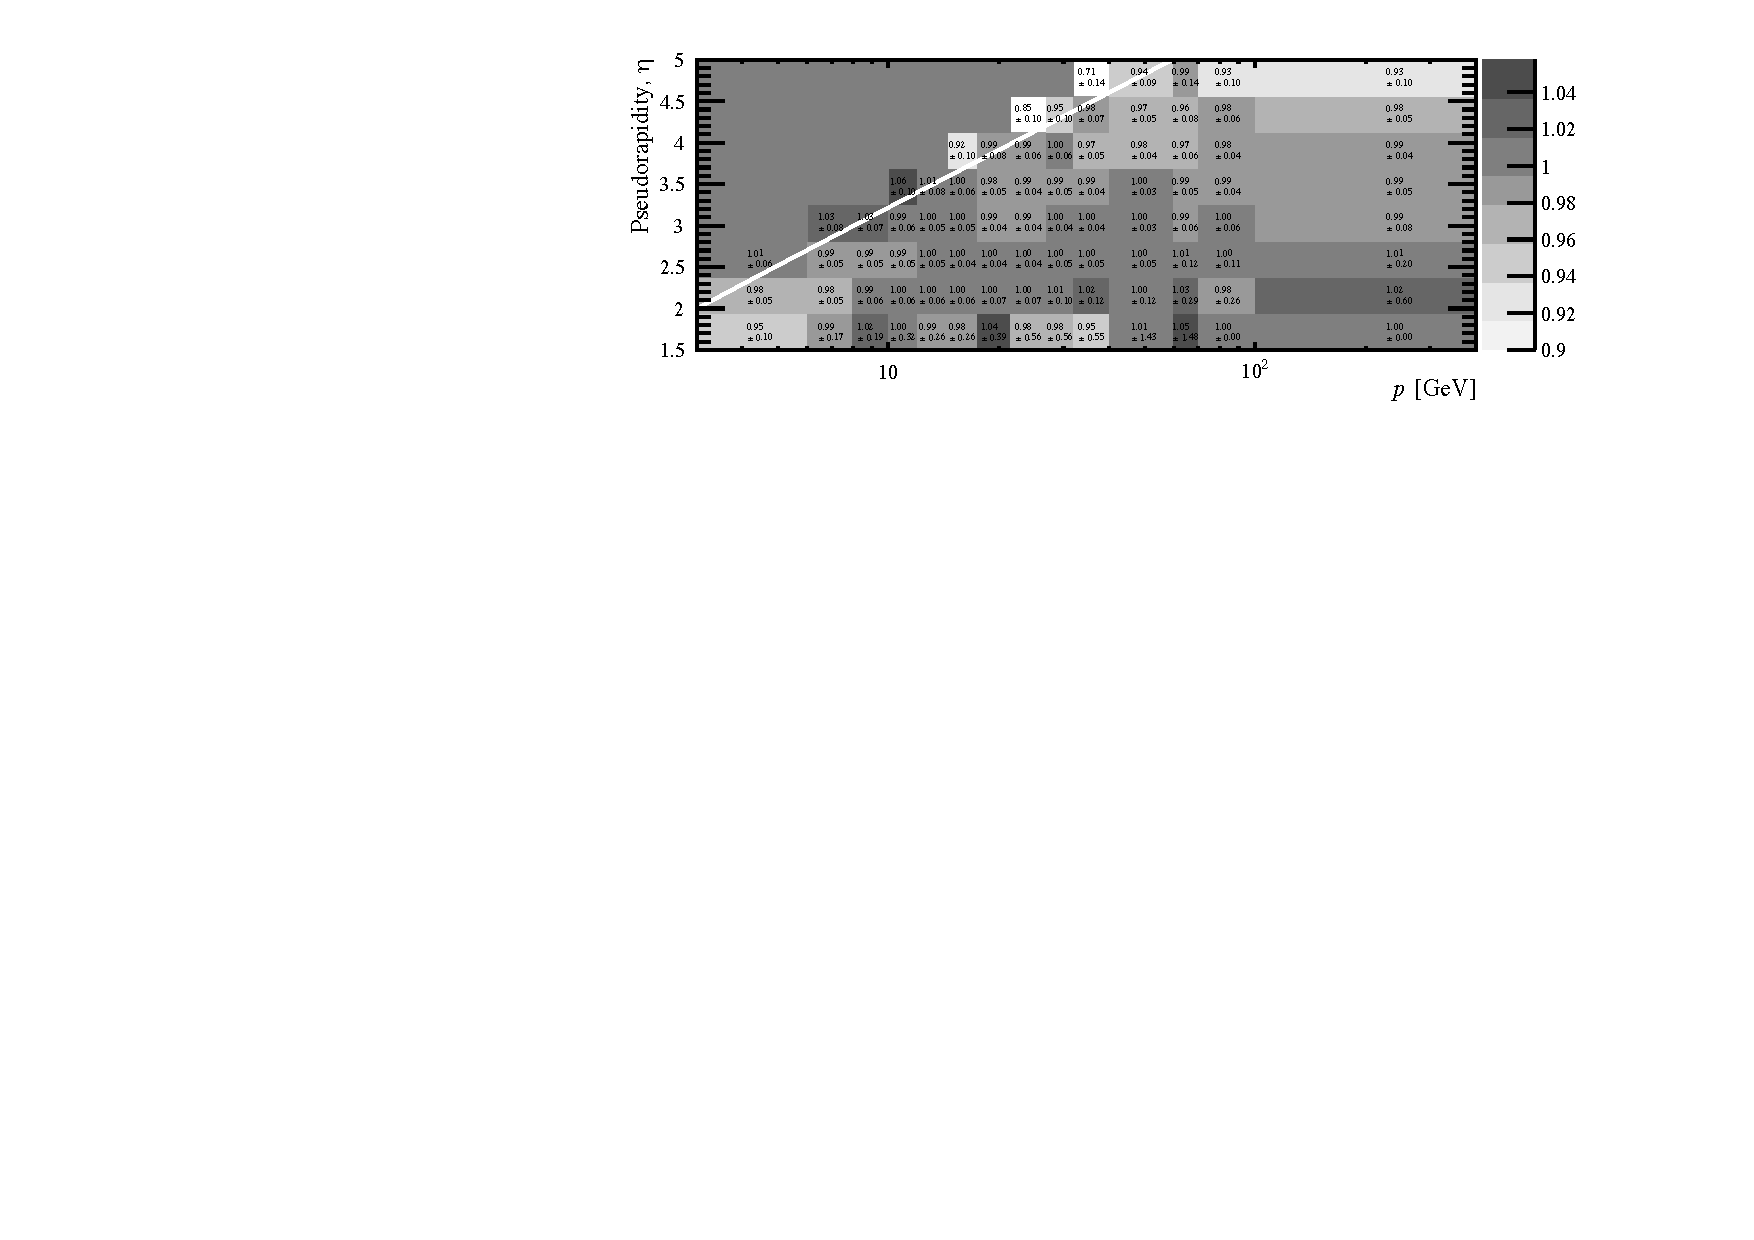
\includegraphics[height=0.23\textheight]{muoneff}
  \end{center}
  \caption[Corrections for {\tt isMuon} and tracking efficiency in simulation]
  {
    The ratio of efficiencies for (top) tracking, and (bottom) \ismuon between data and simulation.
    Simulated tracks in simulation are reweighted according to their momentum and psudorapidity.
    For the lower plot, the calibration sample does not contain muons with $\pt<800\mev$, this
    geometric threshold is indicated by the white line.
  }
  \label{fig:hhh:trackeff}
\end{figure}

\begin{figure}[t]
  \begin{center}
    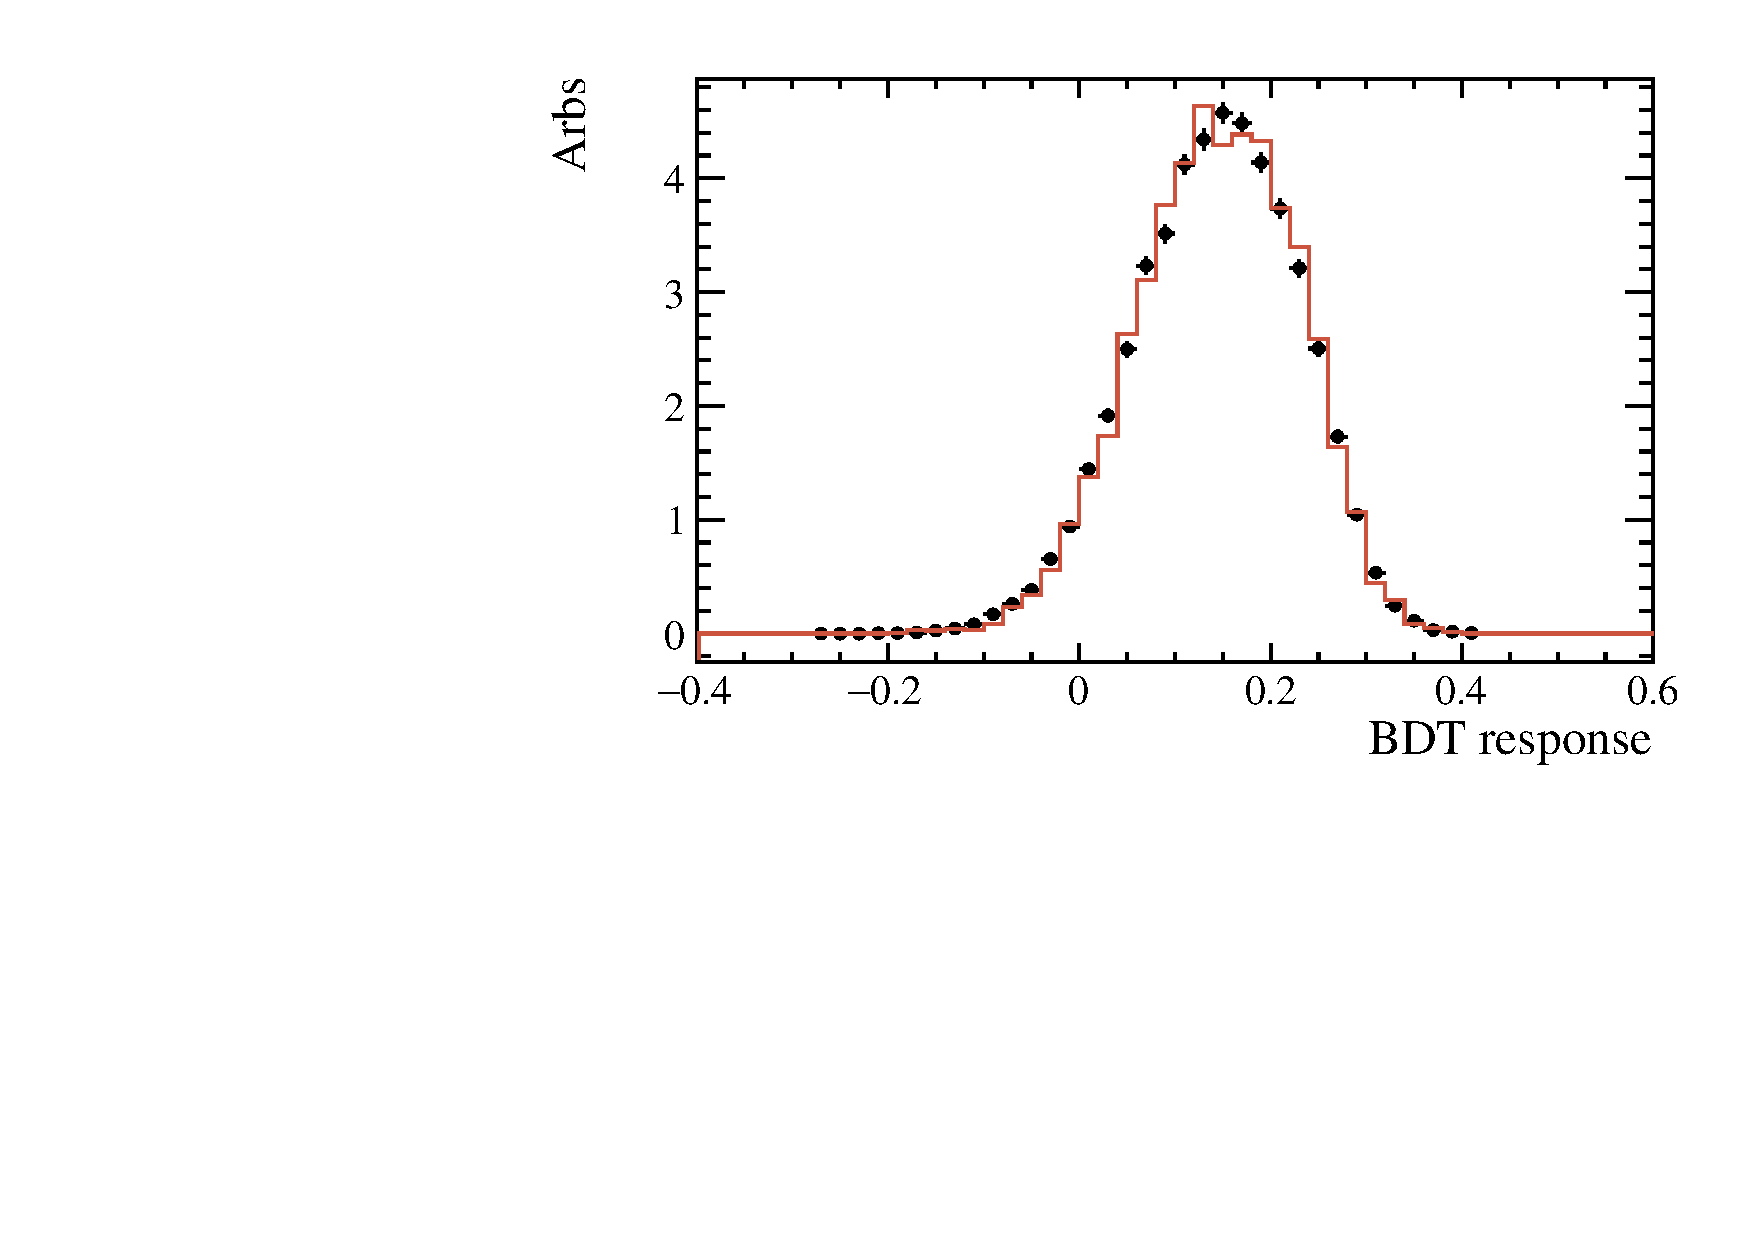
\includegraphics[width=0.48\textwidth]{bdt_k1jpsi}
    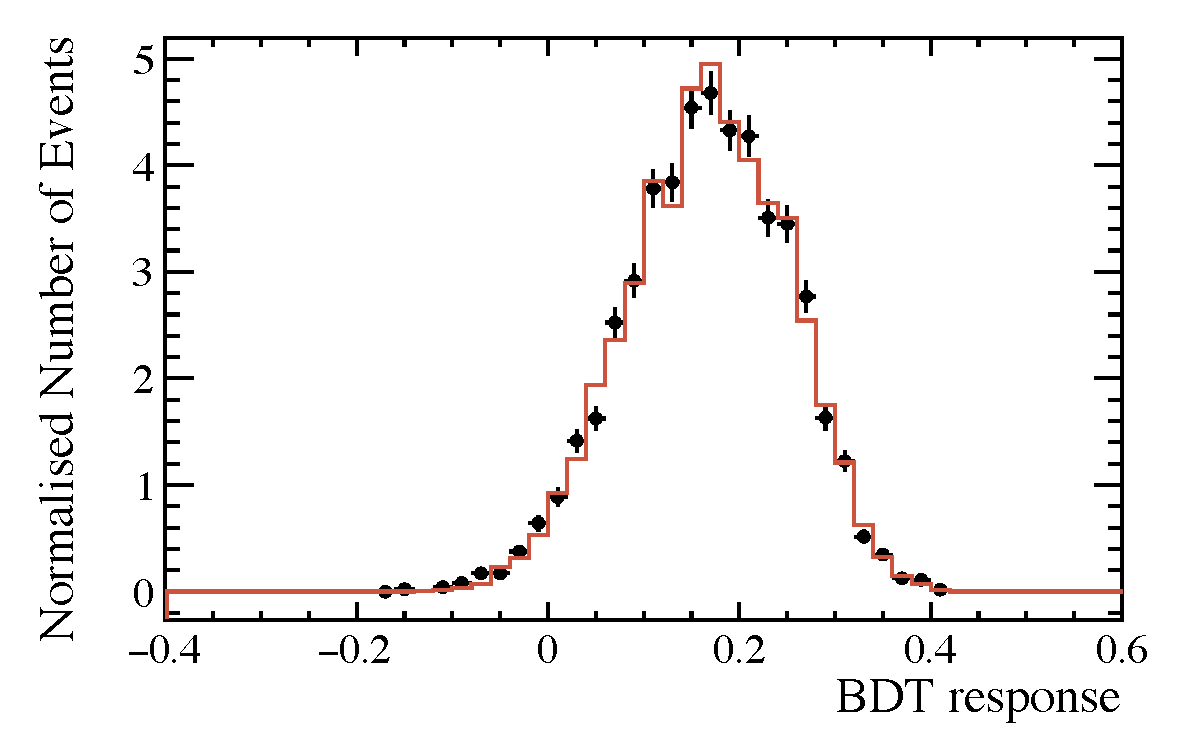
\includegraphics[width=0.48\textwidth]{bdt_psi2sk}
    \caption[Distributions of BDT response in data and simulation]
    {
      Distributions of the \BDT for data (black points) and simulation (red line) for the decay
      (left) \decay{\Bp}{\jpsi\kone{1270}}
      (right) \btopsitwosk.
    }
    \label{fig:kpipi:bdt}
  \end{center}
\end{figure}

Once the simulation has been corrected, the total efficiency, \eff{tot} was calculated for each
normalization and signal mode using simulated events.
The value for \eff{tot} is calculated to be $\eff{gen}\times\eff{reco\&sel}\times\eff{trig}$, where:
\eff{gen} is the generator selection efficiency;
\eff{reco\&sel} is the reconstruction and selection efficiency;
\eff{trig} trigger efficiency.
The generator efficiency defines the probability that a \Bp decays into daughter particles which
all pass through the \lhcb detector acceptance, and is approximately $15\pc$ for each signal and
normalization channel.

%relating to the probabliity of all tracks passing throught the \lhcb dectecor volume;
%Efficiencies for the normalization modes
%$\eff{reco\&sel\&trig}(\btopsitwosk)=(0.4123\pm0.0026)\,\%$, and
%$\eff{reco\&sel\&trig}(\btojpsiphik)=(2.1121\pm0.0013)\,\%$, are calculated

%$\eff{tot}(\btokpipimumu)$,
%$\eff{tot}(\btophikmumu)$, and
%must be made in order to determine the branching fractions for the decays \btokpipimumu and
%\btophikmumu.

%For the decays \btopsitwosk and \btojpsiphik the physics models are well defined, and simulation of
%these events is strainghtforward.
%However, the lack of a model for the inclusive decay \btokpipimumu necessitates an approximation
%must be made with regards to decay model.
%An appropriate choice is the physics model where the \kpipi comes via the \kone{1270} resonance,
%from \Ref{Hatanaka:2008gu} and $\thetakone=34^\circ$.


Since efficiency calculations require reliable simulated samples of decays, accurate physics
models must, or should, be used.
This raises a dilemma deciding how to calculate the efficiency of the signal decays \btokpipimumu
and \btophikmumu, because no physics models exist for them.
For the decay \btokpipimumu, an appropriate choice
was the physics model for \decay{\Bp}{\kone{1270}\mumu}
from \Ref{Hatanaka:2008gu} and $\thetakone=34^\circ$, because this was assumed to be a dominant
contribution.
As there is no available physics model for the decay \btophikmumu, simulated events are produced
using a phasespace model.
These models introduce systematic uncertainties, which are discussed in \Sec{ssec:kpipi:syst} and
\Sec{ssec:phik:syst}.
The efficiencies for signal decays in each \qsq bin are shown in \Fig{fig:hhh:effs}.
Reliable physics models exist for the normalization channels, which have efficiencies measured to
be $\varepsilon(\btopsitwosk)=(0.41\pm0.01)\pc$ and $\varepsilon(\btojpsiphik)=(2.11\pm0.01)\%$
the inefficiency of the former is due to the soft pions from the \psitwos decay failing \pt
requirements in the stripping.

\begin{figure}[t]
  \begin{center}
    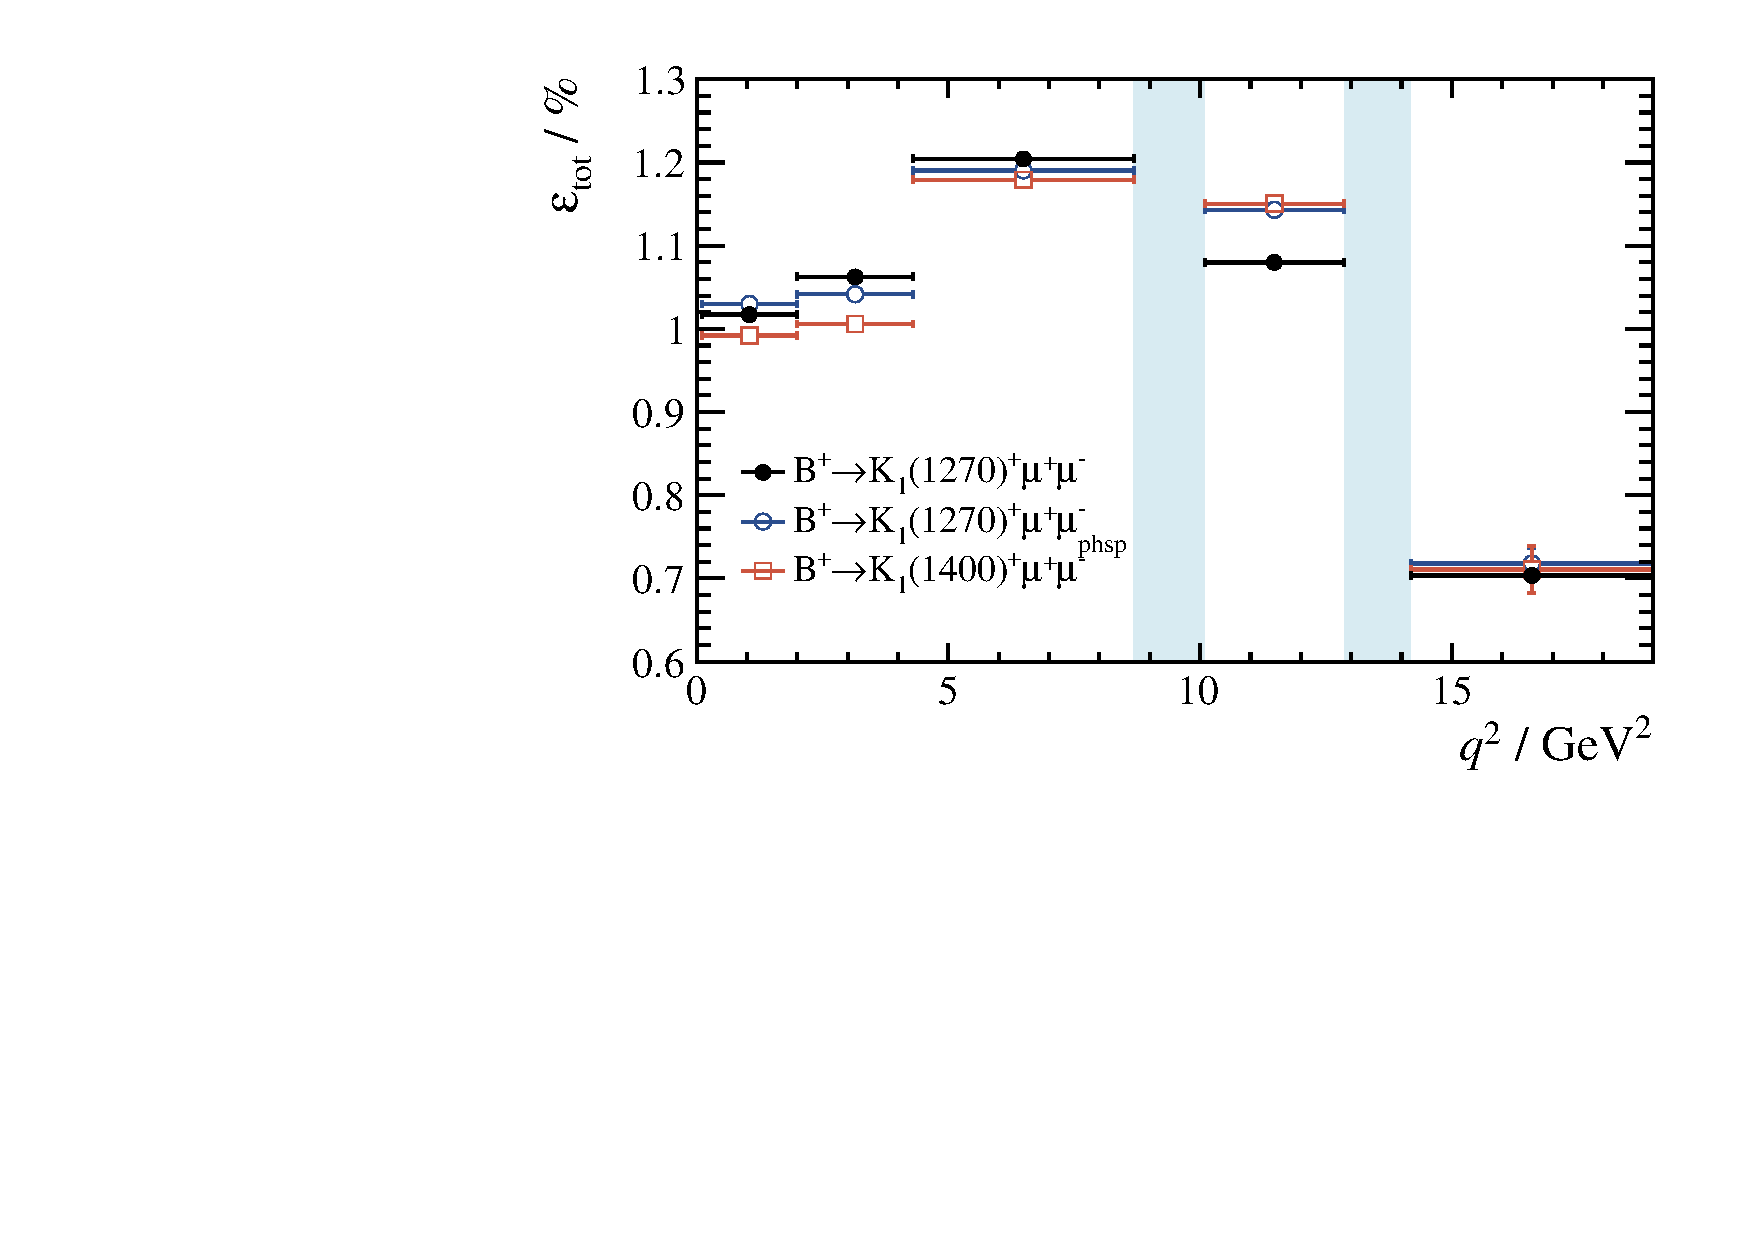
\includegraphics[width=0.48\textwidth]{kpipi_eff}
    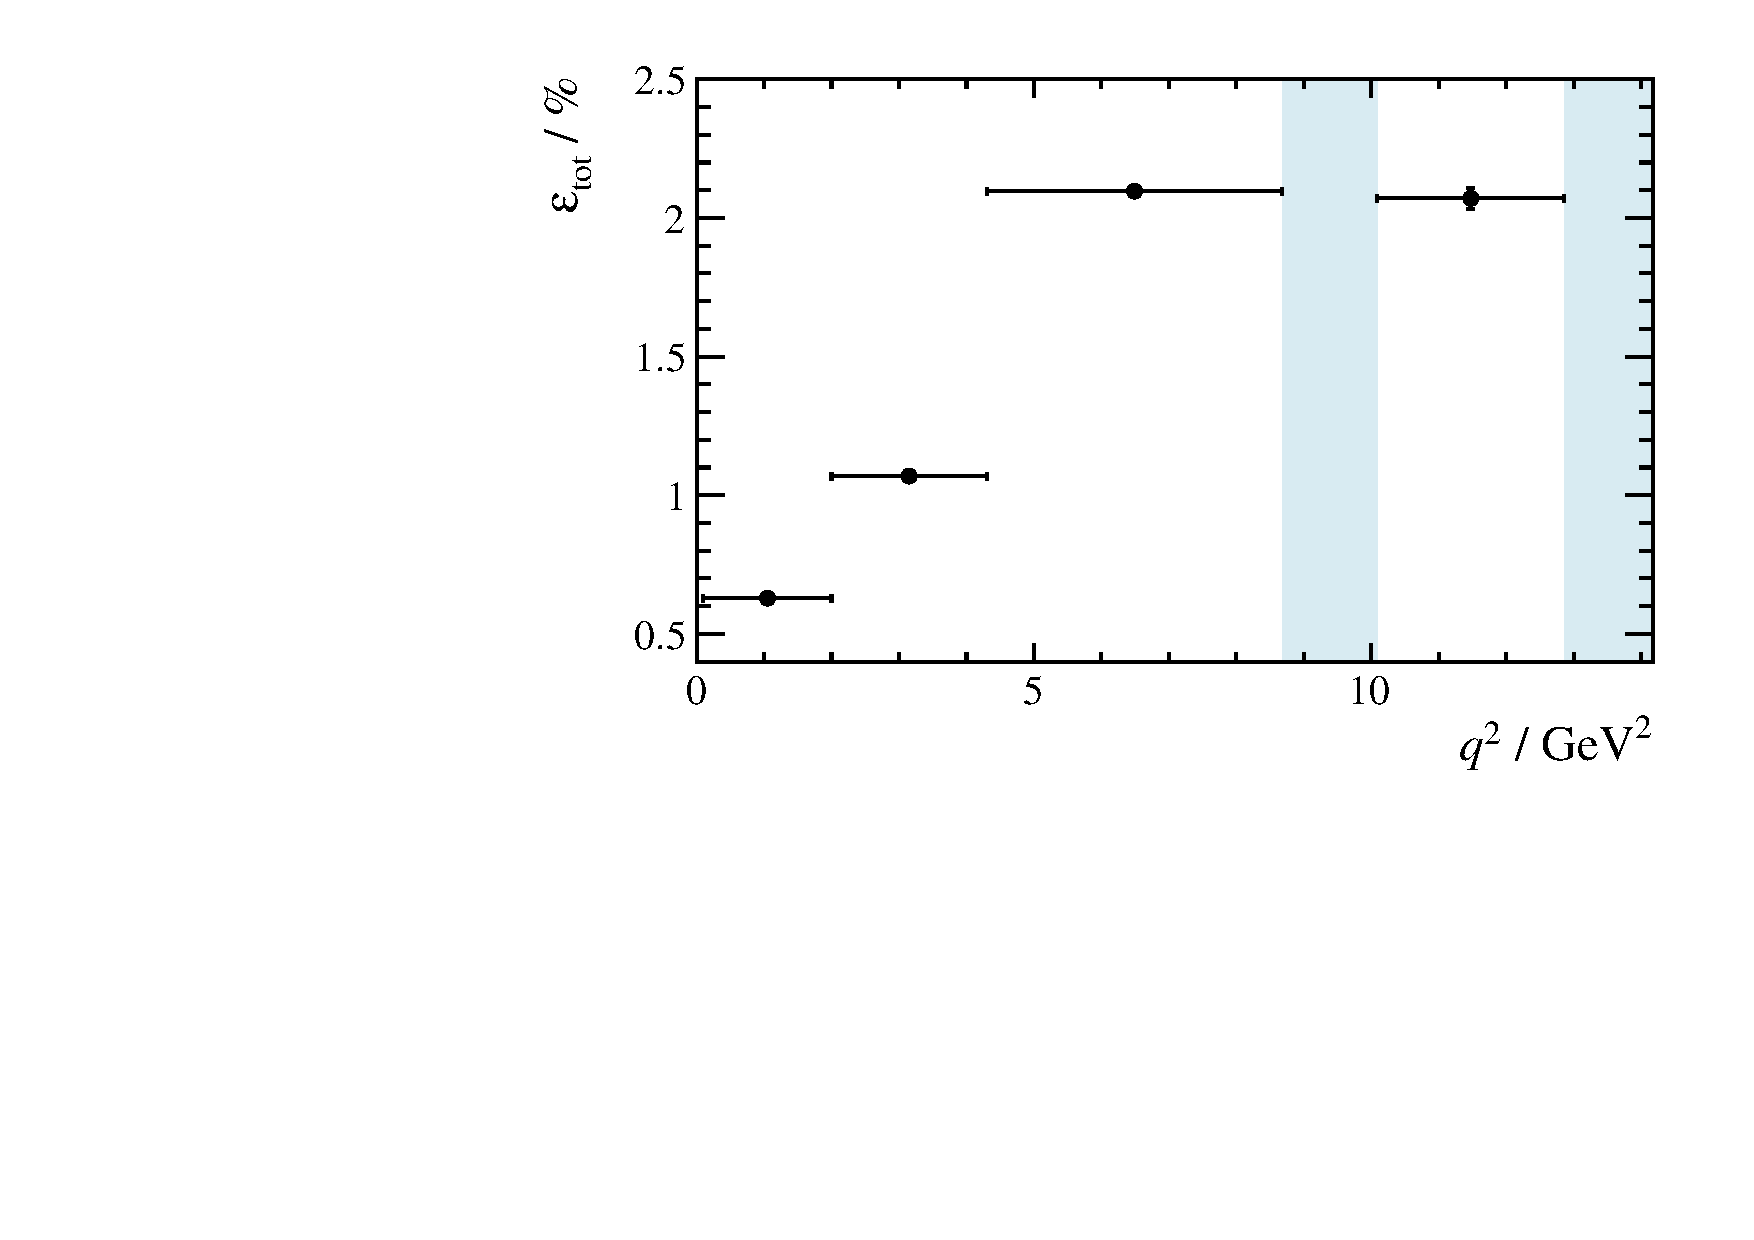
\includegraphics[width=0.48\textwidth]{phik_eff}
    \caption[Efficiency as a funciton of \qsq for \btokpipimumu and \btophikmumu]
    {
      The efficiency of the signal decay
      (left) \btokpipimumu, showing a range of decay models; and
      (right) \btophikmumu in bins of \qsq.
      For the \btophikmumu analysis, there are no events in the $14.18<\qsq<19.00\gevgev$ bin which
      is present in the \btokpipimumu analysis.
      Light blue shaded regions indicate the vetoed \jpsi and \psitwos regions.
    }
    \label{fig:hhh:effs}
  \end{center}
\end{figure}



%\begin{table}
  %\caption{
    %Geometric efficiencies for...
  %}
  %\label{tab:dsphi:geo}
  %\begin{center}
    %\begin{tabular}{lc}\toprule
      %\cellc{Decay} & Geometric efficiency (\%) \\\midrule
      %$\Bp\!\to \jpsi K_1(1270)^+$   & $15.19\pm0.03$ \\
      %$\Bp\!\to \psi(2S) \Kp$   & $15.06\pm0.03$ \\
      %$\Bp\!\to K_1(1270)^+ \mumu$   & $15.14\pm0.02$ \\
      %$\Bp\!\to K_1(1400)^+ \mumu$   & $14.90\pm0.02$ \\
      %$\Bp\!\to K_1(1270)^+ \mumu_\mathrm{phsp}$   & $15.14\pm0.03$ \\
      %$\Bp\!\to\phi\Kp\mumu$   & $16.17\pm0.03$ \\
      %$\Bp\!\to\jpsi\phi\Kp$   & $16.31\pm0.03$ \\
      %\bottomrule
    %\end{tabular}
  %\end{center}
%\end{table}






